\documentclass{report}
% Change "article" to "report" to get rid of page number on title page
\usepackage{amsmath,amsfonts,amsthm,amssymb}
\usepackage{setspace}
\usepackage{Tabbing}
\usepackage{fancyhdr}
\usepackage{lastpage}
\usepackage{extramarks}
\usepackage{chngpage}
\usepackage{soul,color}
\usepackage{listings}
\usepackage{enumerate}
\usepackage{graphicx,float,wrapfig}
\usepackage{pifont}
\usepackage{graphicx}
\usepackage[english]{babel}
\usepackage{tikz}
\usepackage[]{algorithm2e}
% In case you need to adjust margins:
\topmargin=-0.45in      %
\evensidemargin=0in     %
\oddsidemargin=0in      %
\textwidth=6.5in        %
\textheight=9.0in       %
\headsep=0.25in         %

\title{Assignment 1 - Comp 632 - Machine Learning}

% Homework Specific Information
\newcommand{\hmwkTitle}{Assignment 1}                     % Adjust this
\newcommand{\hmwkDueDate}{Tuesday, January 27 2015}                           % Adjust this
\newcommand{\hmwkClass}{COMP 632}


\newcommand{\hmwkClassInstructor}{Dr. Doina Precup}
\newcommand{\hmwkAuthorName}{Geoffrey Stanley}
\newcommand{\hmwkAuthorNumber}{260645907}
\newcommand{\Pp}{\mathbb{P}}
\newcommand{\Ev}{\mathbb{E}}
\newcommand{\cov}{\text{Cov}}
\newcommand{\Z}{\mathbb{Z}}
\newcommand{\R}{\mathbb{R}}
\newcommand{\dd}{\, \mathrm{d}}

% Setup the header and footer
\pagestyle{fancy}                                                       %
\lhead{\hmwkAuthorName}                              %
\chead{}
\rhead{\hmwkClass: \hmwkTitle}                                          %

\lfoot{}
\cfoot{}                                                                %
\rfoot{Page\ \thepage\ of\ \pageref{LastPage}}                          %
\renewcommand\headrulewidth{0.4pt}                                      %
\renewcommand\footrulewidth{0.4pt}                                      %

% This is used to trace down (pin point) problems
% in latexing a document:
%\tracingall
\definecolor{mygreen}{rgb}{0,0.6,0}
\lstset{commentstyle=\color{mygreen}, frame=single,  language=R, showspaces=false, showstringspaces=false}

%%%%%%%%%%%%%%%%%%%%%%%%%%%%%%%%%%%%%%%%%%%%%%%%%%%%%%%%%%%%%
% Make title
\title{\vspace{2in}\textmd{\textbf{\hmwkClass:\ \hmwkTitle}}\\
\normalsize\vspace{0.1in}\small{Due\ on\ \hmwkDueDate}\\
\vspace{0.1in}\large{\textit{Presented to \hmwkClassInstructor}}\vspace{3in}}
\date{}
\author{\textbf{\hmwkAuthorName}\\
    \textbf{Student ID: \hmwkAuthorNumber}}
%%%%%%%%%%%%%%%%%%%%%%%%%%%%%%%%%%%%%%%%%%%%%%%%%%%%%%%%%%%%%

\begin{document}
\maketitle
\section*{Question 1}
\subsection*{A)}
See source code.
\subsection*{B)}
Let $a$ be a vector equal to $[1/max_i |x_j|, ..., 1/max_i |x_n|]$. And let $A$
be a matrix such that $A=aI$. Substituting $X$ by $AX$ in the closed form regression
algorithm we obtain:
\begin{equation}
  \begin{aligned}
  2(AX)^TAXw &= 2(AX)^TY \\
  2AX^TAXw &= 2AX^TY \\
  X^TAXw &= X^TY \\
  Aw &= (X^TX)^{-1}X^TY \\
  \end{aligned}
\end{equation}
As such, we can conclude that normalization is equivalent to multiplying the $w$
vector by some scalar.
\subsection*{C)}
See source code.
\subsection*{D)}
\subsection*{E)}
\begin{center}
    \begin{tabular}{| l | l | l | l | l | l | l | l |}
    \hline
    Fold & 1 & 2 & 3 & 4 & 5 & Avg & Std \\ \hline
    Training Error & 6.6514 & 19.2372 & 64.0957 & 3.5362 & 7.9715 & &  \\ \hline
    Testing Error & 12.0617 & 65.2324 & 63.7457 & 242.0755 & 27.4566 & &  \\ \hline
    Best Hypothesis Class & 3 & 2 & 5 & 5 & 3 & & \\ \hline
    \end{tabular}
\end{center}
\begin{center}
    \begin{tabular}{| l | l |}
    \hline
    Fold & Weights \\ \hline
    1 & 51.6240,   -5.6394,   -0.9195,  117.3091,
         -31.5193,   -1.9346,   -2.8364 \\ \hline
    2 & 61.5754,  119.5093,  -43.5034,   -0.3571,
          -5.0867 \\ \hline
    3 & 23.7598,  -38.3909,  -44.6193,   71.8402,
          79.5440,  -36.2471,   -7.3942,  119.6915,
         -31.7799,    0.9384,   -2.675 \\ \hline
    4 & 56.9424,  -22.7079, -108.6892,   37.0749,
         112.6876,  -13.6251,  -10.9835,  118.9107,
         -32.4987,   -1.3683,   -2.5827 \\ \hline
    5 & 35.4915,    0.8967,    2.4318,  111.0603,
         -29.3260,   -1.0296,   -2.9383 \\ \hline
    \end{tabular}
\end{center}
\subsection*{F)}
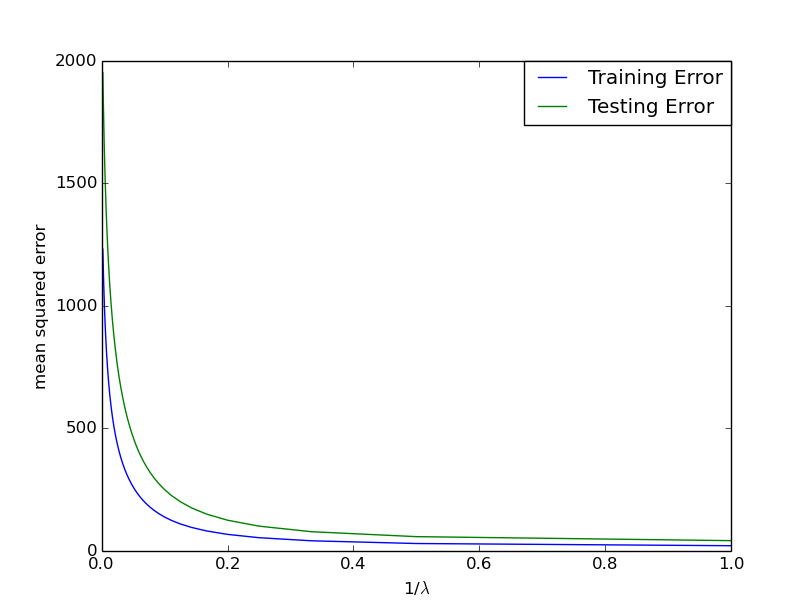
\includegraphics[width=250pt, keepaspectratio=true]{error.png}
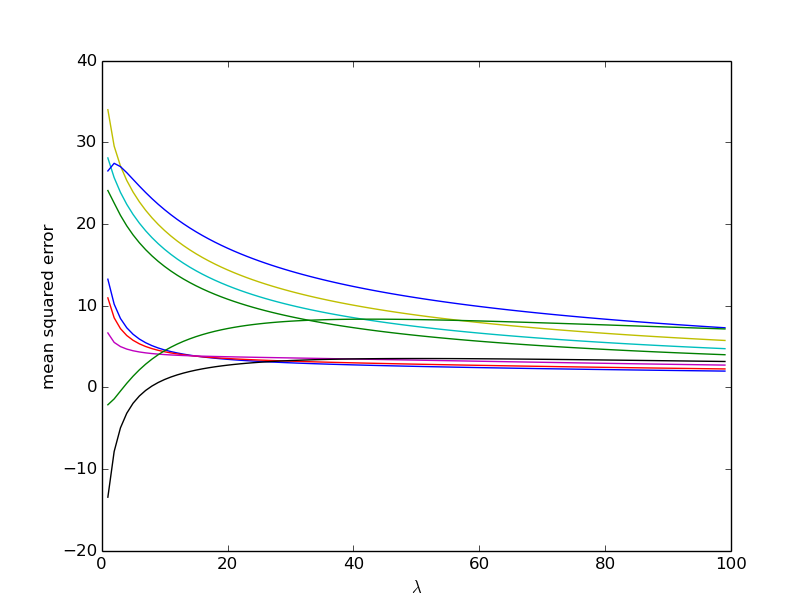
\includegraphics[width=250pt, keepaspectratio=true]{weights.png}

\section*{Question 2}
When simplifying the maximum likelihood equation for a regression whose variables
maintain a constant normal distribution we are able to obtain the sum-squared-error
function. However, when the standard deviation varies from one variable to another
this simplification is no longer achievable.
  \begin{equation}
     L(w) = \prod_{i=1}^{m} \frac{1}{\sqrt{2\pi\sigma_i^2}}e ^ {-\frac{1}{2}\left(\frac{y_i-h_w(x_i)}{\sigma_i}\right)^2}
  \end{equation}

  \begin{equation}
     \log L(w) = \sum_{i=1}^{m} \log \left(\frac{1}{\sqrt{2\pi\sigma_i^2}}\right)
     - \sum_{i=1}^{m} \frac{1}{2}\left(\frac{y_i-h_w(x_i)}{\sigma_i}\right)^2
  \end{equation}

  \begin{equation}
     \log L(w) = \sum_{i=1}^{m} \log \left((2\pi)^{-1/2}\sigma_i^{-1}\right)
     - \sum_{i=1}^{m} \frac{1}{2}\left(\frac{y_i-h_w(x_i)}{\sigma_i}\right)^2
  \end{equation}

  \begin{equation}
     \log L(w) = -\frac{1}{2} \log(2\pi)
     - \sum_{i=1}^{m} \log \sigma_i
     - \sum_{i=1}^{m} \frac{1}{2}\left(\frac{y_i-h_w(x_i)}{\sigma_i}\right)^2
  \end{equation}

\begin{equation}
     \frac{\partial}{\partial w_j} \log L(w)
     = \frac{\partial}{\partial w_j} \left(-\frac{1}{2} \log(2\pi)
     - \sum_{i=1}^{m} \log \sigma_i
     - \sum_{i=1}^{m} \frac{1}{2}\left(\frac{y_i-h_w(x_i)}{\sigma_i}\right)^2\right)
\end{equation}

\begin{equation}
     \frac{\partial}{\partial w_j} \log L(w) =
     - \sum_{i=1}^{m} \frac{x_i}{\sigma_i}\left(\frac{y_i-h_w(x_i)}{\sigma_i}\right)
\end{equation}

Simplying further while converting standard deviation to variance. Where $\sigma^2 = \Omega$.

\begin{equation}
     \frac{\partial}{\partial w_j} \log L(w) =
     \sum_{i=1}^{m} \frac{x_iy_i}{\Omega_i}
     - \sum_{i=1}^{m}\frac{h_w(x_i)x_i}{\Omega_i}
\end{equation}

\begin{equation}
     \frac{\partial}{\partial w_j} \log L(w) =
     X^T\Omega^{-1}Y - wX^T\Omega^{-1}X
\end{equation}

Now setting the gradient to zero.

\begin{equation}
     0 =X^T\Omega^{-1}Y
     - wX^T\Omega^{-1}X
\end{equation}

\begin{equation}
     w^* = (X^T\Omega^{-1} X)^{-1} X^T\Omega^{-1} Y
\end{equation}


\section*{Question 3}
Given the following huberized loss function:
\begin{equation}
  L_H(w, \delta) = \left\{
  \begin{array}{l l}
    (y_i - w^Tx_i)^2 / 2 & \quad \text{if }  | y_i - w^Tx_i | \leq \delta\\
    \delta | y_i - w^Tx_i | - \delta^2 / 2 & \quad \text{otherwise}

  \end{array} \right.\end{equation}


\subsection*{A)}
Find the derivative:

\begin{equation}
  \frac{\partial}{\partial w} L_H(w, \delta) = \left\{
  \begin{array}{l l}
    \frac{\partial}{\partial w} \left((y_i - w^Tx_i)^2 / 2 \right)& \quad \text{if }  | y_i - w^Tx_i | \leq \delta\\
    \frac{\partial}{\partial w} \left(\delta | y_i - w^Tx_i | - \delta^2 / 2\right) & \quad \text{otherwise}

  \end{array} \right.\end{equation}
  \\

The equation $| y_i - w^Tx_i |$ is equivalent to $\sqrt{( y_i - w^Tx_i )^2}$ as such
the derivative becomes:

  \begin{equation}
    \frac{\partial}{\partial w} L_H(w, \delta) = \left\{
    \begin{array}{l l}
      - x_i (y_i - w^Tx_i)  & \quad \text{if }  | y_i - w^Tx_i | \leq \delta\\
      - x_i \delta \frac{y_i - w^Tx_i}{| y_i - w^Tx_i |}  & \quad \text{otherwise}

    \end{array} \right.\end{equation}
    \\

The expression $\frac{y_i - w^Tx_i}{| y_i - w^Tx_i |}$ is equivalent to the sign
of $y_i - w^Tx_i$ as such the derivative can be written as:

\begin{equation}
  \frac{\partial}{\partial w} L_H(w, \delta) = \left\{
  \begin{array}{l l}
    - x_i (y_i - w^Tx_i) & \quad \text{if }  | y_i - w^Tx_i | \leq \delta\\
    - x_i \delta sign ( y_i - w^Tx_i ) & \quad \text{otherwise}

  \end{array} \right.\end{equation}
  \\

Where $sign(y_i - w^Tx_i)$ is replaced by 1 or -1 depending on whether the result of the
equation is positive or negative.

\subsection*{B)}
The algorithm was implemented in python source code and is defined as function
GradientDescent.
\\
\begin{algorithm}[H]
 \KwData{a dataset containing features and targets, learning rate, lambda, delta}
 \KwResult{a weight vector }

 initialize weights to 1 or a random numbers\;

 \While{max iterations not achieved}{
   initialize gradient = 0\;
  \While{not at the last row of the data array}{

    hypothesis = dot product (weights , row of features)\;

    \eIf{$| y_i - w^Tx_i | \leq delta$}{

      loss = hypothesis - row of targets\;
      J = dot product ( transpose of the row features, loss )\;
      gradient += J + lambda/2 * dot product(transpose of weights, weights)\;

     }{
     loss = hypothesis - row of targets\;
     \eIf{loss is negative}{
       gradient += delta * row of features
     }{
       gradient -= delta * row of features
     }
    }

    go to the next row\;
  }
  \If{gradient * learning rate is smaller then desired precision}{
    return weights\;
  }

  weights = weights + (learning rate) * gradient
 }
 return weights\;
 \caption{Gradient descent using huber loss function}
\end{algorithm}
\subsection*{C)}


\section*{Question 4}

  \begin{equation}
    h_{w1,...wk}(x)
    = \prod_{k=1}^{K}\phi_k(x)
  \end{equation}
Where:
  \begin{equation}
    \phi_k(x) = e^{w_k^Tx}
    = e^{\sum_{i=1}^m w_{ik}x_i}
  \end{equation}
Replacing $\phi_k(x)$

  \begin{equation}
    h_{w1,...wk}(x)
    = \prod_{k=1}^{K}e^{\sum_{i=1}^m w_{ik}x_i}
  \end{equation}

  \begin{equation}
    \log h_{w1,...wk}(x)
    = \sum_{k=1}^{K} \sum_{i=1}^m w_{ik}x_i
  \end{equation}

  \begin{equation}
    \frac{\partial}{\partial w} \log h_{w1,...wk}(x)
    = \frac{\partial}{\partial w} \left(\sum_{k=1}^{K} \sum_{i=1}^m w_{ik}x_i\right)
  \end{equation}

  \begin{equation}
    \frac{\partial}{\partial w} \log h_{w1,...wk}(x)
    =  \sum_{i=1}^m x_i
  \end{equation}

\end{document}
